\documentclass{article}
% \documentclass{llncs}
\usepackage{amsmath,amsfonts,url,graphicx,xcolor}
% \graphicspath{ {./images/} }

\begin{document}
\definecolor{yellow}{HTML}{FFFBEB}
\pagecolor{yellow}


\title{
	Zero Knowledge Proof of Location\\
	\small{
	Platin Yellow Paper\\
	Draft}
}
\author{Lionel Wolberger, Vadym Fedyukovych}
% \institute{Platin.io}
\maketitle

\abstract{
Many location based services authorize a user by assessing whether or not the user is within a given range of the service.
To assess this range, systems request the user's geospatial coordinates, and often store them for later analysis.
We describe a system where the service authorization is based on a zero knowledge verification of a commitment.
The commitment has no geographical coordinate data, yet can be reliably verified to prove that the user is within range of the service eligibility.
The service has the assurance required to deliver the service while having zero knowledge of the user's geographical coordinates.
}
\section{Zero Knowledge Proof of Location}

We present two sets of equations with a graphical illustration followed by notes and decisions. 

The illustration describes a location based service with a radius that defines the range of that service.
Two users are shown colored green and red, the green user inside the radius and the red user, outside.
The diagram illustrates parameters that are significant to the zero knowledge proof. 

The equations are presented in two sets and specify the steps required to perform the full protocol, from commitment to verification.
This protocol allows a verifier to test whether position committed is inside or outside the radius of the service area.
Both interactive  and non-interactive protocols are defined, each presented as a series of equations. 

The notes and decisions section records issues related to the protocol and illustration.
Each note discusses a mathematical decision that we have made.
Some of these decisions are not yet reflected in the equations and protocols shared in this paper. 

A git repository is associated with this paper.
C++ reference code can be found there enabling testing and efficiency metrics. 

This zero knowledge proof of location protocol is sufficient for many use cases, efficient, supports large scale analytics, and preserves users' privacy.

\begin{figure}
  \centering
  \def\svgwidth{\columnwidth}
  \input{range_proof.pdf_tex}
\caption{Two users with a predefined radius. green node and a red node are positioned in relation to a circle with a predefined radius. The Pan airdrop is described by circular geometry with a center and radius. A node has three significant parameters: a distance, radius and difference.}
\label{fig-rangeproof}
\end{figure}

%\begin{figure}[!htb]
%	\hspace*{-2cm}
%	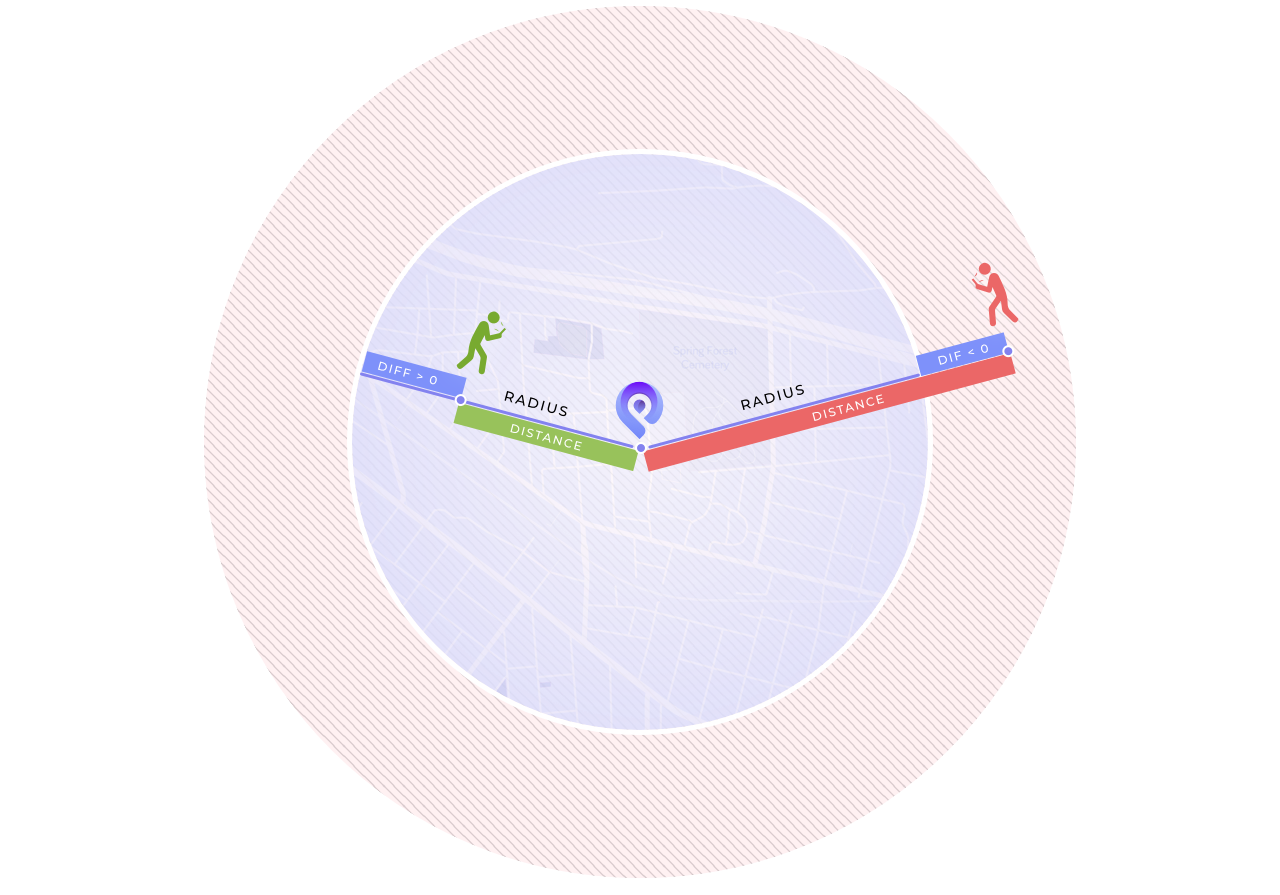
\includegraphics[scale=.3]{zkp_range_proof}
%	\caption{Two users request authorization for a location based service. The center of the circle and its preset radius define a range within which users are to be authorized for the service. With data known only to itself, each user calculates a mathematical commitment based on its radius, distance and difference.  For green the difference is greater than zero. For red the difference is less than zero. The mathematical commitment is verified by applying the zero knowledge protocol below, without revealing the user's geospatial coordinates.}
%\end{figure}

% %%%%%%%%%%%%%%%%%%%%%%%%%%%%%%%%%%%%%%%%%%%%%
\begin{figure}[!htb]
\begin{tabular}{|p{\linewidth}|}
\hline

Common input of Prover and Verifier is
  commitment $s_U$ to node location~\eqref{cmt-up},
  airdrop location $(x_l, y_l, z_l)$ and
  threshold $d^2$ (integers),
  parameters $(N, g, g_x, g_y, g_z, g_r, \{h_j\})$.
\begin{gather}
\label{cmt-up}
  s_U = g_x^{x_n} g_y^{y_n} g_z^{z_n} g^{r} \pmod{N}
\end{gather}
Private input of Prover is
  node location $(x_n, y_n, z_n)$ (integers) and location commitment randomness~$r$,
  four numbers~$\{a_j\}$ calculated
% with Rabin-Shallit algorithm
  according to~\eqref{eq-distn}.
\\
Statement being proved is
\begin{gather}
\label{eq-distn}
  d^2 - ((x_n - x_l)^2 + (y_n - y_l)^2) + (z_n - z_l)^2) = \sum_{j=1}^4 a_j^2
\end{gather}
Protocol runs as follows:
\begin{enumerate}
\item
  Prover picks random $\{\alpha_j\}, \eta, \gamma, \beta_x, \beta_y, \beta_z, \beta_r, \rho_0, \rho_1$,
  produces $f_0, f_1$, sends $b_0, b_1, t_a, s_a, t_n$:
\begin{gather}
  f_0 = -(\beta_x^2 + \beta_y^2 + \beta_z^2) - \sum_{j=1}^4 \alpha_j^2   \\
  f_1 = -( (x_n - x_l) \beta_x  + (y_n - y_l) \beta_y  + (z_n - z_l) \beta_z) - \sum_{j=1}^4 a_j \alpha_j   \\
%
  t_n = g_x^{\beta_x} g_y^{\beta_y} g_z^{\beta_z} g^{\beta_r} ,   \;
  s_a = g^{\gamma} \prod_{j=1}^4 h_j^{a_j},   \;
  t_a = g^{\eta} \prod_{j=1}^4 h_j^{\alpha_j} \\
  b_0 = g^{f_0} g_r^{\rho_0},  \;
  b_1 = g^{2 f_1} g_r^{\rho_1} \pmod{N}
\end{gather}
%
\item
  Verifier chooses and sends his challenge $c$
\item
  Prover produces and sends responses
\begin{gather}
  X_n = c x_n + \beta_x,  \;
  Y_n = c y_n + \beta_y,  \;
  Z_n = c z_n + \beta_z,  \;
  R = c r + \beta_r   \\
  A_j = c a_j + \alpha_j, \;
  R_a = c \gamma + \eta,   \;
  R_d = c \rho_1 + \rho_0
\end{gather}
%
\item
  Verifier accepts if
\begin{gather}
\label{verf-linear}
  g_x^{X_n} g_y^{Y_n} g_z^{Z_n} g^{R} s_U^{-c} = t_n, \quad
  g^{R_a} (\prod_{j=1}^4 h_j^{A_j}) s_a^{-c} = t_a \\
\label{verf-distn}
  g^{c^2 d^2 - ((X_n - c x_l)^2 + (Y_n - c y_l)^2 + (Z_n - c z_l)^2) - (A_1^2 + A_2^2 + A_3^2 + A_4^2)} g_r^{R_d} = b_1^{c} b_0  \pmod{N}
\end{gather}
\end{enumerate}
\\
\hline
\end{tabular}
\caption{Private location verification protocol, interactive version}
\label{ip_fig}
\end{figure}

% %%%%%%%%%%%%%%%%%%%%%%%%%%%%%%%%%%%%%%%%%%%%%
\begin{figure}[!htb]
\begin{tabular}{|p{\linewidth}|}
\hline

Input of Prover is
  location commitment~$s_U$~\eqref{cmt-up},
  location $(x_n, y_n, z_n)$ and random $r$ to open this commitment,
  airdrop location $(x_l, y_l, z_l)$,
  threshold $d^2$,
  parameres $(N, g, g_x, g_y, g_z, g_r, h_j)$
  and public information $pubp$.
\\
Non-interactive proof is produced as follows:
\begin{enumerate}
\item
  Prover calculates $a_1 \dots a_4$ from locations and threshold,
  picks random $\{\alpha_j\}, \eta, \gamma, \beta_x, \beta_y, \beta_z, \beta_r, \rho_0, \rho_1$,
  produces $t_n, s_a, t_a, b_0, b_1$:
\begin{gather}
  t_n = g_x^{\beta_x} g_y^{\beta_y} g_z^{\beta_z} g^{\beta_r}, \;
  s_a = g^{\gamma} (\prod_{j=1}^4 h_j^{a_j}),  \;
  t_a = g^{\eta} (\prod_{j=1}^4 h_j^{\alpha_j}) \pmod{N}
\end{gather}
\begin{gather}
  \tilde f_0 = \beta_x^2 + \beta_y^2 +\beta_z^2 + \alpha_1^2 + \alpha_2^2 + \alpha_3^2 + \alpha_4^2  \\
  \tilde f_1 = (x_n - x_l) \beta_x  + (y_n - y_l) \beta_y  + (z_n - z_l) \beta_z + a_1 \alpha_1 + a_2 \alpha_2 + a_3 \alpha_3 + a_4 \alpha_4 \\
  b_0 = g^{\tilde f_0} g_r^{\rho_0},   \quad
  b_1 = g^{2 \tilde f_1} g_r^{\rho_1} \pmod{N}
\end{gather}

\item
  Prover produces his challenge with a hash function
  from text representation of commitments generated at previous step and public information:
\begin{gather}
  c = H(t_n || s_a || t_a || b_1 || b_0 || s_U || pubp)
\end{gather}

\item
  Prover produces responses:
\begin{multline}
  X_n = -c x_n + \beta_x,  \;
  Y_n = -c y_n + \beta_y,  \;
  Z_n = -c z_n + \beta_z,   \;
  R = -c r + \beta_r   \\
  A_j = -c a_j + \alpha_j, \;
  R_a = -c \gamma + \eta,   \;
  R_d = -c \rho_1 + \rho_0
\end{multline}
\end{enumerate}
Non-interactive proof is
$(c, X_n, Y_n, Z_n, R, \{A_j\}, R_a, R_d, s_a, b_1)$.
\\
Proof verification:
\begin{multline}
\label{verf-chash}
  F_d = ((X_n + c x_l)^2 + (Y_n + c y_l)^2 + (Z_n + c z_l)^2) + (A_1^2 + A_2^2 + A_3^2 + A_4^2) - c^2 d^2 \\
  H(g_x^{X_n} g_y^{Y_n} g_z^{Z_n} g^{R} s_U^{c} ||
    s_a ||
    g^{R_a} (\prod_{j=1}^4 h_j^{A_j}) s_a^{c} ||
    b_1 ||
    g^{F_d} g_r^{R_d} b_1^c ||
    s_U ||
    pubp)
  = c
\end{multline}
\\
\hline
\end{tabular}
\caption{Location proof generation and verification, non-interactive version}
\label{ni_fig}
\end{figure}



\section{Notes and Decisions}

Notes and decisions capture issues related to zero knowledge proofs of location and are presented in no particular order. Some of the topics discussed relate to our general approach to zero knowledge proofs, and do not directly reflect the equations or protocols above. The contents of notes and decisions may be integrated with the main body of the paper in future. 

\subsection{Some Definitions}
\label{sect-definitions}
Node proves the statement "distance is within a threshold" (less or equal)
for node coordinates $(x_n, y_n, z_n)$,
given location $(x_l, y_l, z_l)$,
and some threshold $d$ (all integers):
\begin{gather}
\label{eq-distn-cp}
  d^2 - ((x_n - x_l)^2 + (y_n - y_l)^2 + (z_n - z_l)^2) = a_1^2 + a_2^2 + a_3^2 + a_4^2
\end{gather}
We rely on 4-squares Lagrange theorem to prove equality statement~\cite{Lipmaa03}.
Proofs for integer relations are possible in hidden group order setup.

\subsection{Proof Setup}

Let $g$ be a generator of a proper group of a hidden order,
and $h$ be a group element (Pedersen commitment scheme).
We use multiplicative group of invertible residue classes modulo a composite $n$ such that
$n=pq$, $p=2p'+1$, $q=2q'+1$ and $p, q, p', q'$ primes~\cite{Idemix}.

\subsection{Representation-Based Commitment}
Following U-Prove, consider commitment scheme resulting in a single group element:
\begin{gather}
\label{cmt-up-cp}
  s_U = g_x^{x_n} g_y^{y_n} g_z^{z_n} g^{r}
\end{gather}
where $g_x, g_y, g_z$ are group elements, and $r$ is a random.
This scheme admits a proof of knowledge with the same responses required form threshold location verification.
This scheme can be extended with additional components. % like set of wireless station% name-power pairs.

\subsection{Two-Level Commitment}
To achieve expected properties of Merkle-tree based scheme while keeping an option
to run location proof protocols,
representation-based commitments could be leaves of Merkle tree.

\subsection{A Not-at-Location Proof}

Proving a negative location statement is a valid usecase,
that could be demonstrated with ``not at the grocery store'' scenario.
Rather that proving ``distance is smaller than''~\eqref{eq-distn-cp},
complementary ``is larger'' proof is given. % as follows:
In the following, we only show changes required to the main protocol.
\begin{gather}
\label{eq-distn-more}
  ((x_n - x_l)^2 + (y_n - y_l)^2 + (z_n - z_l)^2) - d^2 = a_1^2 + a_2^2 + a_3^2 + a_4^2  \\
\label{verf-distn-more}
  g^{((X_n - c x_l)^2 + (Y_n - c y_l)^2 + (Z_n - c z_l)^2 ) - c^2 d^2 - (A_1^2 + A_2^2 + A_3^2 + A_4^2)} h^{R_a} = b_1^{c} b_0 
\end{gather}
\begin{multline}
\label{eq-coeff-more}
  f_V(v) = f_2 v^2 + f_1 v + f_0 = \\
  (((v x_n + \beta_x) - v x_l)^2 +
   ((v y_n + \beta_y) - v y_l)^2 +
   ((v z_n + \beta_z) - v z_l)^2)
  - v^2 d^2 \\
  - ((v a_1 + \alpha_1)^2 +
     (v a_2 + \alpha_2)^2 +
     (v a_3 + \alpha_3)^2 +
     (v a_4 + \alpha_4)^2)
\end{multline}

\subsection{Logical-OR Threshold Location}

Consider a franchise operating multiple stores,
and a usecase of proving location is ``at Starbucks'' without telling which one of $K$ known.
We define each such store with it's center $(x_k, y_k, z_k)$ and radius (size)~$d_k$, $k \in [1 .. K]$.
We elaborate basic threshold proof such that prover can produce
4-squares representation for center-size of some store $k=p$,
and pick arbitrary 4-tuples for all other stores $k \ne p$.
\begin{multline}
\label{eq-distn-or}
  \prod_{k=1}
    ((d_k^2 - ((x_n - x_k)^2 + (y_n - y_k)^2 + (z_n - z_k)^2) \\
     - (a_{1, k}^2 + a_{2, k}^2 + a_{3, k}^2 + a_{4, k}^2)) = 0
\end{multline}
Verifier is testing that polynomial $f_{KV}(v)$ is of degree at most $2K-1$, not $2K$.
\begin{multline}
  f_{KV}(v) = \sum_{j=0}^{2K} f_j v^j = \\
  \prod_{k=1}^{K} (
    v^2 d_k^2 - (((v x_n + \beta_x) - v x_k)^2 +
               ((v y_n + \beta_y) - v y_k)^2 +
               ((v z_n + \beta_z) - v z_k)^2)  \\
        - ((v a_{1,k} + \alpha_1)^2 +
           (v a_{2,k} + \alpha_2)^2 +
           (v a_{3,k} + \alpha_3)^2 +
           (v a_{4,k} + \alpha_4)^2) )
\end{multline}


\bibliographystyle{plain}
% \bibliographystyle{splncs}
\bibliography{private_location_verification}

%\appendix
\end{document}
